\let\negmedspace\undefined
\let\negthickspace\undefined
\documentclass[journal]{IEEEtran}
\usepackage[a5paper, margin=10mm, onecolumn]{geometry}
%\usepackage{lmodern} % Ensure lmodern is loaded for pdflatex
\usepackage{tfrupee} % Include tfrupee package

\setlength{\headheight}{1cm} % Set the height of the header box
\setlength{\headsep}{0mm}     % Set the distance between the header box and the top of the text

\usepackage{gvv-book}
\usepackage{gvv}
\usepackage{cite}
\usepackage{amsmath,amssymb,amsfonts,amsthm}
\usepackage{algorithmic}
\usepackage{graphicx}
\usepackage{textcomp}
\usepackage{xcolor}
\usepackage{txfonts}
\usepackage{listings}
\usepackage{enumitem}
\usepackage{mathtools}
\usepackage{gensymb}
\usepackage{comment}
\usepackage[breaklinks=true]{hyperref}
\usepackage{tkz-euclide} 
\usepackage{listings}
% \usepackage{gvv}                                        
\def\inputGnumericTable{}                                 
\usepackage[latin1]{inputenc}                                
\usepackage{color}                                            
\usepackage{array}                                            
\usepackage{longtable}                                       
\usepackage{calc}                                             
\usepackage{multirow}                                         
\usepackage{hhline}                                           
\usepackage{ifthen}                                           
\usepackage{lscape}
\usepackage{circuitikz}
\tikzstyle{block} = [rectangle, draw, fill=blue!20, 
    text width=4em, text centered, rounded corners, minimum height=3em]
\tikzstyle{sum} = [draw, fill=blue!10, circle, minimum size=1cm, node distance=1.5cm]
\tikzstyle{input} = [coordinate]
\tikzstyle{output} = [coordinate]


\begin{document}

\bibliographystyle{IEEEtran}
\vspace{3cm}

\title{2.10.28}
\author{AI25BTECH11039-Harichandana Varanasi}
 \maketitle
% \newpage
% \bigskip
{\let\newpage\relax\maketitle}

\renewcommand{\thefigure}{\theenumi}
\renewcommand{\thetable}{\theenumi}
\setlength{\intextsep}{10pt} % Space between text and floats


\numberwithin{equation}{enumi}
\numberwithin{figure}{enumi}
\renewcommand{\thetable}{\theenumi}



\date{}

\begin{document}
\maketitle


\section*{Question}
\textbf{Q 2.10.28.} For non-zero vectors $\vec{a},\ \vec{b},\ \vec{c}$, the relation
\begin{equation}
\label{eq:q-21028}
\Bigl|(\vec{a}\times\vec{b})\cdot\vec{c}\Bigr|
=\|\vec{a}\|\,\|\vec{b}\|\,\|\vec{c}\|
\end{equation}
holds if and only if
\begin{enumerate}[label=(\alph*)]
  \item $\vec{a}\cdot\vec{b}=0,\ \ \vec{b}\cdot\vec{c}=0$
  \item $\vec{b}\cdot\vec{c}=0,\ \ \vec{c}\cdot\vec{a}=0$
  \item $\vec{c}\cdot\vec{a}=0,\ \ \vec{a}\cdot\vec{b}=0$
  \item $\vec{a}\cdot\vec{b}=\vec{b}\cdot\vec{c}=\vec{c}\cdot\vec{a}=0$
\end{enumerate}

\begin{solution}
Let
\begin{align}
A=\myvec{\vec{a}&\vec{b}&\vec{c}},\qquad 
G=A^\top A
=\myvec{
\vec{a}^\top\vec{a} & \vec{a}^\top\vec{b} & \vec{a}^\top\vec{c}\\
\vec{b}^\top\vec{a} & \vec{b}^\top\vec{b} & \vec{b}^\top\vec{c}\\
\vec{c}^\top\vec{a} & \vec{c}^\top\vec{b} & \vec{c}^\top\vec{c}}
\label{eq:gram-matrix}
\end{align}
be the column and Gram matrices of $\vec{a},\vec{b},\vec{c}$.
The given magnitude equals $\abs{\det A}$, so
\begin{align}
\abs{\det A}^{\,2}=(\det A)^2
=\det\!\paren{A^\top A}
=\det G .
\label{eq:det-square}
\end{align}
By Hadamard’s inequality for the positive semidefinite matrix $G$,
\begin{align}
\det G
\le (\vec{a}^\top\vec{a})\,
   (\vec{b}^\top\vec{b})\,
   (\vec{c}^\top\vec{c})
= \|\vec{a}\|^{2}\,\|\vec{b}\|^{2}\,\|\vec{c}\|^{2},
\label{eq:hadamard-bound}
\end{align}
with equality \emph{iff} $G$ is diagonal, i.e., the columns of $A$ are pairwise orthogonal:
\begin{align}
\vec{a}^\top\vec{b}=0,\qquad
\vec{b}^\top\vec{c}=0,\qquad
\vec{c}^\top\vec{a}=0 .
\label{eq:orth}
\end{align}
Taking square roots in 4.2 and 4.3 yields
\begin{align}
\abs{\det A}
= \|\vec{a}\|\,\|\vec{b}\|\,\|\vec{c}\|
\iff
4.4 holds.
\label{eq:final}
\end{align}
Hence, the correct option is \(\boxed{\text{(d)}}\).
\end{solution}



     \begin{figure}[h!]
\centering
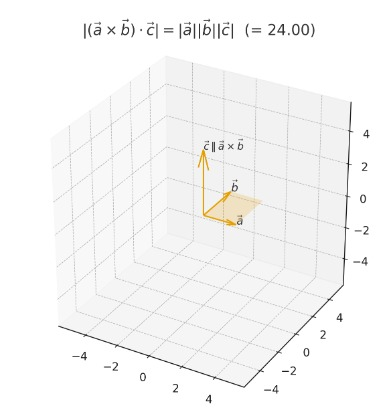
\includegraphics[width=0.5\linewidth]{figs/2.10.28.jpeg}
\caption{Illustration of $|( \vec a\times\vec b)\cdot\vec c|=|\vec a|\,|\vec b|\,|\vec c|$ with $\vec a\perp\vec b$ and $\vec c\parallel(\vec a\times\vec b)$.}


\end{figure}

\end{document}
